\section{Baseline}

The baseline model is DeFMO.\@
Here, the input consists of an RGB image $I \in \mathbb{R}^{H \times W \times 3}$ of the foreground blurred FMO with height $H$ and width $W$, and another RGB Image $B \in \mathbb{R}^{H \times W \times 3}$ of the background.
The desired output is a deblurred rendering of the FMO for $N$ sub-frames.
The $t$\textsuperscript{th} sub-frame is an RGBA image $R_t \in \mathbb{R}^{H \times W \times 4}$ consisting of an RGB part $F_t \in \mathbb{R}^{H \times W \times 3}$ for the sharp appearance of the FMO, and an alpha matting mask $M_t \in \mathbb{R}^{H \times W}$ which segments the FMO from the background.

Since the motion blur in the input image is due to movement of the FMO with long exposure time, we should be able to reconstruct the input image using the output sub-frames.
This can be achieved by mimicking how a camera would capture the FMO.\@
For this, \citet{blatting-1,blatting-2} introduce the blurring and matting (blatting) equation:
\begin{equation}
    I = H \ast F + (1 - H \ast M) B \label{eq:blatting}
\end{equation}
Here, $F$ is the sharp foreground appearance of the object, $M$ is the segmentation mask, and $H$ is the blur kernel.
$H$ identifies the object's trajectory such that $||H|| = 1$.

DeFMO generalizes this with the following model:
\begin{equation}
    I_{t_0:t_1} = \int_{t_0}^{t_1} F_t M_t dt + \left( 1 - \int_{t_0}^{t_1} M_t dt \right) B \label{eq:defmo-blatting}
\end{equation}
Here, the trajectory blur kernels $H_t$ aren't disentangled, because they are just Dirac deltas.

\begin{figure}
    \centering
    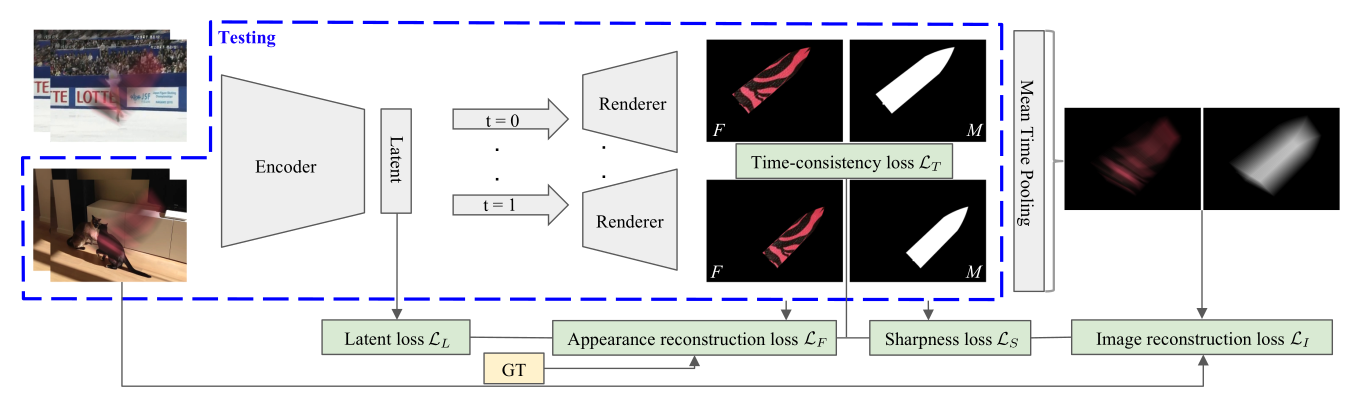
\includegraphics[width=\textwidth]{images/defmo-arch.png}
    \caption{Architecture of DeFMO.}%
    \label{fig:defmo-arch}
\end{figure}

\paragraph{Architecture}
DeFMO uses an encoder to encode $I$ and $B$ into a latent vector $X \in \mathbb{R}^K$.
The encoder is a CNN that takes both $I$ and $B$ concatenated along the channel axis.
A renderer takes $X$ and time indices $t_0, t_1, \ldots, t_{N-1}$ to output the $N$ sub-frames.
This is also a CNN that uses sub-pixel convolutions~\citep{pixelshuffle}, also known as pixel shuffles, for upsampling.
An illustration of the architecture is shown in Figure~\ref{fig:defmo-arch}.

\subsection{Training losses}
    DeFMO uses a wide variety of losses to optimize the model.
    These consist of the output reconstruction loss ($\mathcal{L}_F$), the input reconstruction loss (based on Equation~\ref{eq:defmo-blatting}) ($\mathcal{L}_I$), and losses to constraint the output to have smooth movements in time ($\mathcal{L}_T$), sharp objects ($\mathcal{L}_S$), and invariance to the background ($\mathcal{L}_L$).
    Therefore, the total loss is a weighted sum of these losses:
    \begin{equation}
        \mathcal{L}_{\mathrm{DeFMO}} = \mathcal{L}_F + \alpha_I \mathcal{L}_I + \alpha_T \mathcal{L}_T + \alpha_S \mathcal{L}_S + \alpha_L \mathcal{L}_L
    \end{equation}

    \paragraph{Appearance reconstruction loss}
    $\mathcal{L}_F$ is the supervised loss for the output sub-frames.
    However, since the model has to generate movement based on a single image as the input, the movement can be in either the same direction as the ground-truth or the opposite.
    Therefore, the supervised loss $\mathcal{L}_R$ is calculated for both directions, and $\mathcal{L}_F$ is the minimum of these:
    \begin{equation}
        \mathcal{L}_F({\{ R_t, \tilde{R}_t \}}_1^N) = \frac{1}{N} \min \left( \sum_{t=1}^N \mathcal{L}_R(R_t, \tilde{R}_t) dt, \sum_{t=1}^N \mathcal{L}_R(R_t, \tilde{R}_{1-t}) dt \right)
    \end{equation}

    $\mathcal{L}_R$ for the output rendering $R_t$ and the ground-truth $\tilde{R}_t$ at time $t$ is calculated as:
    \begin{equation}
    \begin{split}
        \mathcal{L}_R(R_t = (F_t, M_t), \tilde{R}_t = (\tilde{F}_t, \tilde{M}_t)) &= \mathcal{L}_1(M_t, \tilde{M}_t, \tilde{M}_t > 0) + \mathcal{L}_1(M_t, \tilde{M}_t, \tilde{M}_t = 0)\\
        &+ \mathcal{L}_1(F_t M_t, \tilde{F}_t \tilde{M}_t, \tilde{M}_t > 0)
    \end{split}%
    \label{eq:loss-supervised}
    \end{equation}
    where $\mathcal{L}_1(A, B, M)$ is the $\mathcal{L}_1$ loss for images $A$ and $B$ conditioned on the mask $M$:
    \begin{equation}
        \mathcal{L}_1(A, B, M) = \frac{\sum_{i, j} {|| A_{i,j} - B_{i,j} ||}_1 M_{i,j}}{\sum_{i,j} M_{i,j}}
    \end{equation}

    In Equation~\ref{eq:loss-supervised}, the first two terms are for comparing the masks $M_t$ and $\tilde{M}_t$ for the foreground and background (as given by the ground truth) separately.
    The separation is to prevent imbalance due to smaller objects in a large background.
    The third term is for the object, but evaluated only in the foreground to disentangle the mask and the object channels.

    \paragraph{Image reconstruction loss}
    $\mathcal{L}_I$ is just an application of the blatting equation in Equation~\ref{eq:defmo-blatting}.
    Thus, this loss is just the $\mathcal{L}_1$ loss between the blatted image and the input image $I$:
    \begin{equation}
        \mathcal{L}_I({\{ R_t \}}_1^N, I) = {\left|\left| \frac{1}{N} \sum_{t=1}^N F_t M_t + \left( 1 - \frac{1}{N} \sum_{t=1}^N M_t \right) B - I \right|\right|}_1
    \end{equation}

    \paragraph{Time-consistency loss}
    $\mathcal{L}_T$ captures the temporal smoothness of the $N$ output sub-frames.
    Informally, we want the sub-frames for nearby $t$ to be similar to each other.
    This similarity is formalized by the maximum value of the normalized cross-correlation over all pixels.
    Thus, the loss is:
    \begin{equation}
        \mathcal{L}_T({\{R_t\}}_1^N) = 1 - \frac{1}{N-1} \sum_{t=1}^{N-1} \mathrm{maxncc}(R_t, R_{t+1})
    \end{equation}

    \paragraph{Sharpness loss}
    Here, $\mathcal{L}_S$ only focuses on the sharpness of the mask, and not the object contents itself.
    The mask is expected to be binary in most of the image, except at the boundaries.
    However, we simplify this constraint to just enforcing binary values.
    This is expressed by the per-pixel binary entropy $\mathcal{H}_2$ averaged over all $H \times W$ pixels:
    \begin{equation}
        L_S({\{M_t\}}_1^N) =  \frac{1}{NHW} \sum_{t=1}^N \sum_{i=1}^H \sum_{j=1}^W \mathcal{H}_2({[M_t]}_{i,j})
    \end{equation}

    \paragraph{Latent learning loss}
    $\mathcal{L}_L$ aims to constrain the model such that blurred images of the same FMO moving along the same trajectory but in front of different backgrounds generate the output.
    This can be achieved by modelling the latent space such that these images have the same latent representation.
    Thus, DeFMO trains in pairs of such images, and computes $\mathcal{L}_L$ between their latent vectors $X_1, X_2 \in \mathbb{R}^K$as:
    \begin{equation}
        \mathcal{L}_L(X_1, X_2) = \frac{{|| X_1 - X_2 ||}_1}{K}
    \end{equation}

    Note that not all losses used here are unbiased, especially the time-consistency and sharpness losses.
    The ground-truth renderings won't necessarily be the minimum of these losses individually, since the time-consistency loss prefers static sub-frames, and the sharpness loss prefers binary masks everywhere, even on boundaries.
    This brings us to our proposed approach, where we want to overcome these limitations and get more general losses.
